\documentclass{beamer}

\usetheme{Warsaw}
%\usecolortheme{lily} 
\setbeamercolor{frametitle}{bg=blue,fg=yellow} 
%\beamersetaveragebackground{blue!10} 

\newcommand{\supp}{\textrm{{s}upp}
}
\newcommand{\ce}{\mbox{\textnormal{{c}e}}
}
\newcommand{\card}{\mbox{\textnormal{{c}ard}}
}
\newcommand{\rc}{\mbox{\textnormal{rc}}
}
\newcommand{\sig}{\textrm{$\Sigma$Count}
}
\newcommand{\nf}{\mbox{\textnormal{nf$\sigma$-count}}
}
\newcommand{\req}[1]{(\ref{#1})}
\newcommand{\inn}{\mbox{\textnormal{in}}
}
\newcommand{\clm}{\mbox{\textnormal{clm}}
}

\usepackage[utf8]{inputenc}
\usepackage{amssymb}
\usepackage{graphicx} %for eps graphics
\usepackage[T1]{fontenc}
\usepackage[polish]{babel}
\usepackage{txfonts}
\usepackage{array}
\usepackage{graphicx}
\usepackage{caption}
\newcommand{\source}[1]{\caption*{Source: {#1}} }

\title{Kubernetes cluster deployment \\ for production environment}
%\toctitle{Kubernetes cluster deployment for production environment}

\author{Ewa Czechowska \\
 \textbf{Supervisor: }dr hab. inż. Aneta Poniszewska-Marańda}
\institute{Lodz University of Technology}
\date{Łódź, 4th April 2020}

%\begin{frame}{\tableofcontents[currentsection]}
%\begin{frame}{\tableofcontents[currentsubsection]}

\begin{document}
\maketitle

\section{Introduction and definitions}
\subsection{Virtualization and Docker containers}
\begin{frame}{Virtualization - history}%{{{
\begin{center}
\begin{tabular}{@{}  l  l l }
	\begin{figure}
		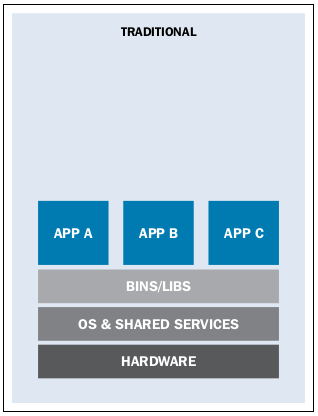
\includegraphics[width=3cm]{figures/virtualization-physical.png}
		\label{fig:virtualization-physical}
	\end{figure} &
	\begin{figure}
		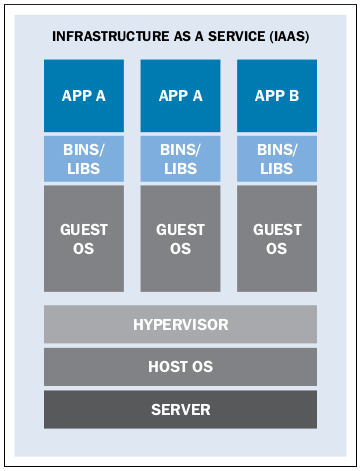
\includegraphics[width=3cm]{figures/virtualization-vms.png}
		\label{fig:virtualization-vms}
	\end{figure} &
	\begin{figure}
		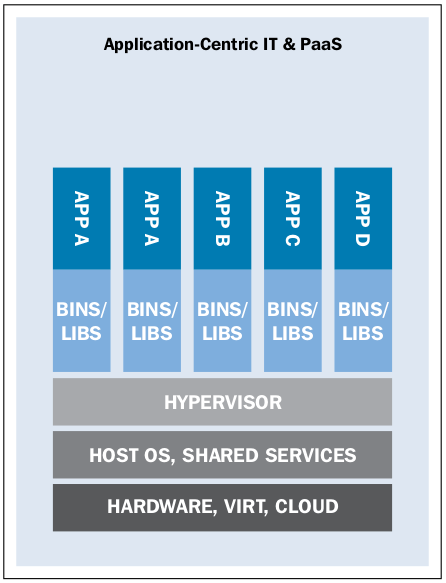
\includegraphics[width=3cm]{figures/virtualization-c.png}
		\label{fig:virtualization-c}
	\end{figure} \\
	\end{tabular}
\end{center}
\tiny{Source: Uphill, Thomas, et. al. \textit{DevOps: Puppet, Docker and Kubernetes}. Packt Publishing, 2017. ISBN 978-1788297615}
\\
\footnotesize{
\begin{enumerate}
	\item Applications were installed on \textbf{physical hardware} directly
	\item Virtualization was invented. \textbf{Virtual Machines (VMs)} have separate OS and provide a safer environment
	\item In 2013 Docker was created as a standard way to manage \textbf{containers}.
\end{enumerate}
}
\end{frame}

	% In order to make this presentation understandable, we need to start with some history.

	% At first all applications were installed on physical hardware directly. This had some drawbacks like: long maintenance cycle, hardware resources were underutilized and also a risk/stress of breaking down the whole host.

	% Then, virtualization was invented to overcome these limitations. Virtual machines were (and still are) emulating the hardware. Each virtual machine has a guest Operating System, which means we can e.g. deploy Windows VM on a laptop with Linux. Virtualization has advantages like: isolation, higher flexibility (we can choose and change how many RAM and how many CPUs we want attached to a VM). However, there are also costs: increased complexity and redundancy. Redundancy: guest OS is redundant. 

	% Then, in 2013, Docker was created as a standard way to manage \textbf{containers}. Docker uses Linux's underlying kernel features which enable containerization. Docker containers support various OSs but  the kernel is shared with the host OS. This leads e.g. to a better utilization of resources (because the kernel is shared among containers).


\begin{frame}{Reasons for using VMs and containers}%{{{
VMs and containers:
\begin{itemize}
\item Provide \textbf{safer, isolated environment} - facilitate experiments
\item Easier to automate, manage and replace
\item \textbf{Reproducible environment}
\item Limit "works on my machine" problem
\item More \textbf{secure}, the firewall can be set to deny any access to host
\item Additional features, e.g. memory replication
\end{itemize}
\end{frame}
%}}}

\begin{frame}{Comparison of Docker containers and VMs}%{{{
\begin{center}
	\begin{flushleft}
	\begin{tabular}{@{}  | c | c | c | @{}}
		\hline
		 & \textbf{Containers} & \textbf{VMs} \\
		 \hline
		 Isolation & Yes, but less & Yes, more \\
		 \hline
		 Pre-baked images & Yes & Yes \\
		 \hline
		Portability across clouds & Yes & No \\
		\hline
		Light-weight & Yes & No \\
		\hline
		Limited OS selection & Yes & No \\
		\hline
		Standardized way of building image & Yes (Dockerfile) & No \\
		\hline
		\end{tabular}
	\end{flushleft}
\end{center}
\tiny{Source: Alonso, Ruben. \textit{Software containerization with Docker}. Bachelor's thesis. Turku University of Applied Sciences, 2017.} \\
\tiny{Source: Saito, Hideto. \textit{DevOps with Kubernetes: Accelerating software delivery with container orchestrators}. Packt Publishing, 2017.}
\end{frame}
%Docker containers and VMs are similar. VMs emulate hardware while containers are an abstract way of packaging software.%
% doing immutable deployment with VM images is costly, because of image sizes and because we have to use custom Configuration Management system
% Standardized way of building such image - for vms a nice solution is using Packer
% Docker instances are lighter-weight. To ship an app as a virtual machine image, you have to bake an entire operating system into the image. With a container, only the app itself has to go inside the container. This translates to a less complicated build process, plus the ability to host many more containers on a single physical server.
%}}}

\begin{frame}{Docker images and Docker containers}%{{{
	\begin{itemize}
		\item \textbf{In order to run (start) a Docker container, a Docker image is needed}
		\item An image is \textbf{a read-only template}. It has some software installed and configured
		\item Each image has a name and a tag - version. Saved in the form of: name:tag
		\item An image may be \textbf{based on other image}.
		\item There are many images available which are open-source and free, e.g. debian:10.3, ubuntu:16.04
		\item It is \textbf{easy to build one's own image}, basing on the available images
	\end{itemize}
	\tiny{Source: \url{https://docs.docker.com}}
\end{frame}

\begin{frame}{Docker image example}%{{{
	\begin{center}
		\begin{figure}
			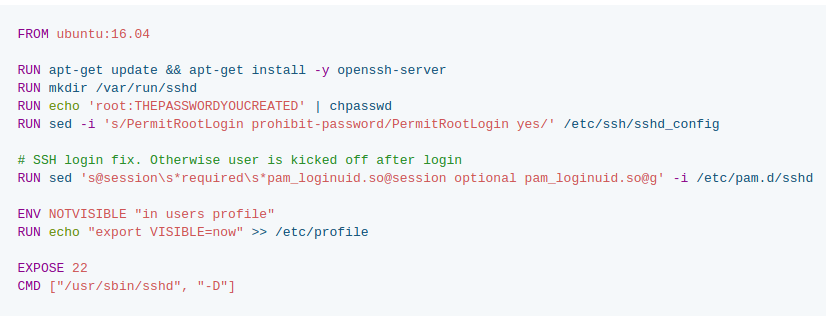
\includegraphics[width=11.5cm]{figures/docker-image.png}
			\label{fig:micro-vs-mono}
		\end{figure} 
		\tiny{Source: \url{https://docs.docker.com/engine/examples/running_ssh_service/}}
		
	\end{center}
\end{frame}

\begin{frame}{Docker image example}%{{{
	\begin{center}
		Build a Docker image:
	\begin{figure}
		
\includegraphics[width=6.5cm]{figures/docker-image-build.png}
		\label{fig:micro-vs-mono}
	\end{figure} \\
	Run the image as a container:\\
	\begin{figure}
		
\includegraphics[width=10cm]{figures/docker-run.png}
		\label{fig:micro-vs-mono}
	\end{figure} 
	\tiny{Source: \url{https://docs.docker.com/engine/examples/running_ssh_service/}}
\end{center}
\end{frame}


\begin{frame}{Deployment options}%{{{
\begin{itemize}
	\item \textbf{On-premises} - local deployment; private cloud
	\item \textbf{In the cloud} - using cloud services providers like: Amazon Web Services, Azure, Google Cloud Platform (GCP)
	\item \textbf{Hybrid} - mix of the two above
\end{itemize}
~\\
~\\
This study focuses on deployment in the cloud.
\end{frame}
%}}}

\subsection{Microservices}
\begin{frame}{Microservices - definition}%{{{
\textbf{Microservices} = A new \textbf{architecture for applications} which evolved as a solution to \textbf{monolith}'s problems.

~\\

\begin{figure}
	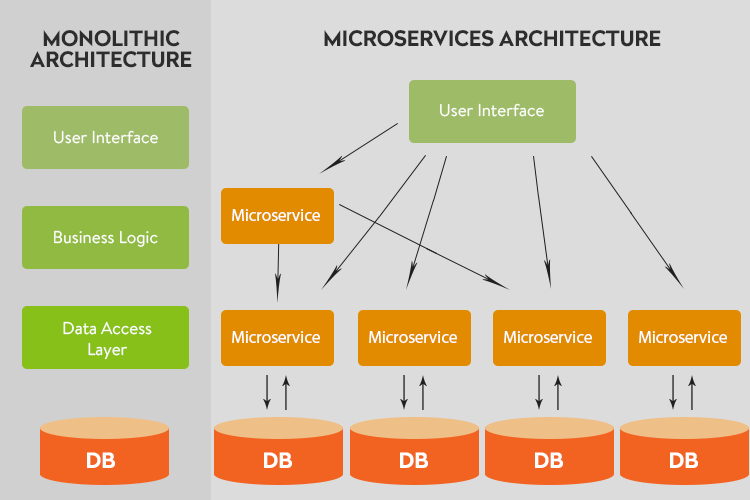
\includegraphics[width=6cm]{figures/Microservices_architecture_vs_monolith.png}
	\label{fig:micro-vs-mono}
\end{figure} 
\tiny{Source: Pogrebnoy, Konstantin, et. al. \textit{Microservices Architecture: to Build or Not to Build}. codetiburon, 2019. [Accessed: 06.04.2020] Available at: \url{https://codetiburon.com/app/uploads/2018/07/Microservices_architecture_vs_monolith.png}} 
\end{frame}
%}}}

\begin{frame}{Advantages of microservices compared to monoliths}%{{{
	\textbf{Advantages of microservices compared to monoliths}:
	\begin{itemize}
		\item Simpler architecture
		\item We can reuse an application
		\item Less context at once
		\item Isolated failures
		\item Smaller and faster deployments
		\item We can use new technology
		\item Scalability
	\end{itemize}
	
	\tiny{Source: Nemer, Joe. \textit{Advantages and Disadvantages of Microservices Architecture}. Cloud Academy, 2019. [Accessed: 06.04.2020] Available at: https://cloudacademy.com/blog/microservices-architecture-challenge-advantage-drawback/} 
	\tiny{Source: Balalaie, Armin, et. al. \textit{Microservices Architecture Enables DevOps: An Experience Report on Migration to a Cloud-Native Architecture}. IEEE Software, 2016, vol. 33.} 
	\end{frame}
	% Improved fault isolation: Larger applications can remain mostly unaffected by the failure of a single module.
	% Scalability: Since your services are separate, you can more easily scale the most needed ones at the appropriate times, as opposed to the whole application. When done correctly, this can impact cost savings.
	%}}}

\begin{frame}{Microservices challenges}%{{{
\begin{itemize}
	\item Communication between services is complex
	\item Global testing is difficult
	\item Debugging problems can be harder
	\item Deployment challengers
	\item Management problems - now there are many services deployed instead of one
\end{itemize}
~\\
\tiny{Source: Nemer, Joe. \textit{Advantages and Disadvantages of Microservices Architecture}. Cloud Academy, 2019. [Accessed: 06.04.2020] Available at: https://cloudacademy.com/blog/microservices-architecture-challenge-advantage-drawback/} 
\end{frame}
%}}}

\subsection{DevOps}
\begin{frame}{The DevOps movement}%{{{
``DevOps is a movement to \textbf{reduce barriers and friction between organizational silos} - development, operations, and other stakeholders involved in planning, building, and running software. Although technology is the most visible (...), it’s \textbf{culture, people, and processes} which have the most impact on flow and effectiveness.``
\\
~\\
\tiny{Source: Morris, Kief. \textit{Infrastructure as Code}. Edition 1. O'Reilly Media, 2016.} 
\end{frame}
%}}}

\begin{frame}{Continuous Delivery (CD)}%{{{
Continuous Delivery helps us to \textbf{incorporate software changes into production environment}, including bug fixes and experiments, safely, quickly in a sustainable way.
\\
The goal is to \textbf{continuously deploy} the software. It is necessary to master this task, so that the deployments and predictable and reliable.
\\
\textbf{Benefits}:
\begin{itemize}
	\item Low risk releases
	\item Faster time to market
	\item Higher quality
	\item Lower costs
\end{itemize}
\tiny{Source: https://continuousdelivery.com/ [Accessed: 06.04.2020]} 
\end{frame}
%}}}

\begin{frame}{Introduction summary}%{{{
Trends related to software deployment:
\begin{itemize}
\item Architectural shift {\bfseries from monolith to microservices}
\item Adoption of {\bfseries Docker containers}
\item Emerging movement: {\bfseries DevOps}
\item Migration {\bfseries from on-premises services to Cloud Native Applications}
\end{itemize}
\end{frame}
%}}}
% \item to satisfy the need for scalability
% \item to decrease the upfront infrastructure investment
% \item to pay only for used infrastructure, not for the allocated part
% \item to utilize resources in a more efficient way
% \item to use reliable infrastructure (thanks to e.g. S3 SLA)

\section{About this study}
\subsection{Table of Contents}
\begin{frame}{Table of Contents}%{{{
\begin{center}
\begin{tabular}{@{}  l  l }
	\begin{figure}
		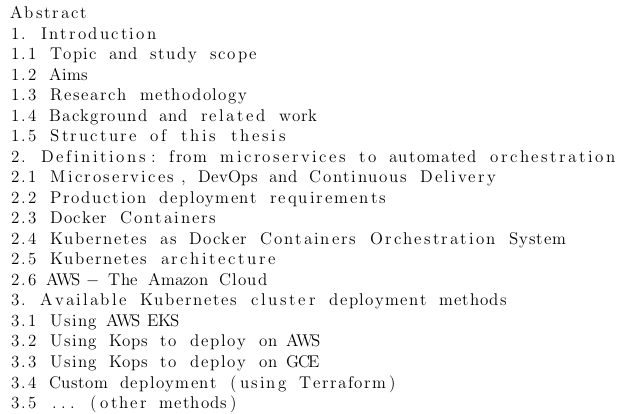
\includegraphics[width=5.5cm]{figures/table-of-c1.png}
		\label{fig:table-of-c1}
	\end{figure} &
	\begin{figure}
		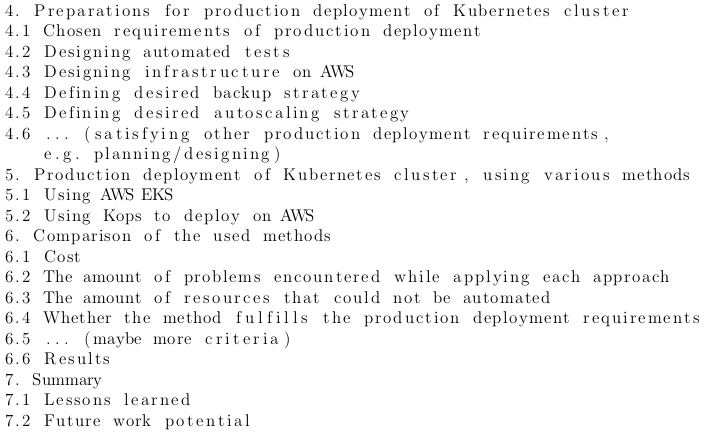
\includegraphics[width=5.5cm]{figures/table-of-c2.png}
		\label{fig:table-of-c2}
	\end{figure} \\
	\end{tabular}
\end{center}
\end{frame}
%}}}


\subsection{1.1 Topic and study scope}	
\begin{frame}{Title again}%{{{
\begin{center}
\LARGE{Kubernetes cluster deployment for production environment}
\end{center}
\end{frame}
%}}}

\begin{frame}{1.1 Topic and study scope - Kubernetes (k8s) - definition}%{{{
\begin{itemize}
\item An open-source system for \textbf{automating deployment, scaling, and management of containerized applications}
\item A platform for managing application containers across multiple hosts
\item First released in 2014
\item Can be \textbf{deployed on many clouds} (AWS, GCP, Azure) or \textbf{on-premises} - unified experience
\item Based on \textbf{15 years of experience} of running production workloads at Google
\item A \textbf{CNCF} graduated project
\end{itemize}
\begin{tabular}{  c c }
\begin{figure}
	
\includegraphics[width=2cm]{figures/kubernetes-logo.png}
	\label{fig:kubernetes-logo}
\end{figure} &
\begin{figure}
	
\includegraphics[width=2cm]{figures/cncf-logo.png}
	\label{fig:cncf-logo}
\end{figure} 
\end{tabular} \\
\tiny{Source: https://kubernetes.io/ [Accessed: 06.04.2020]} \\
\tiny{Source: Saito, Hideto. \textit{DevOps with Kubernetes: Accelerating software delivery with container orchestrators}. Packt Publishing, 2017.}
\end{frame}

\begin{frame}{1.1 Topic and study scope - k8s features}%{{{
\begin{itemize}
	\item Container deployment
	\item Persistent storage
	\item Container health monitoring
	\item Compute resource management
	\item Auto-scaling
	\item High availability by cluster federation
	\item Secret and configuration management
	\item Service discovery and load balancing
\end{itemize}

\tiny{Source: https://kubernetes.io/ [Accessed: 06.04.2020]} 
\tiny{Source: Saito, Hideto. \textit{DevOps with Kubernetes: Accelerating software delivery with container orchestrators}. Packt Publishing, 2017.}
% it's useful
\end{frame}
%}}}

\begin{frame}{1.1 Topic and study scope - topic choice}%{{{
k8s is popular and used by practicioners
\begin{figure}
	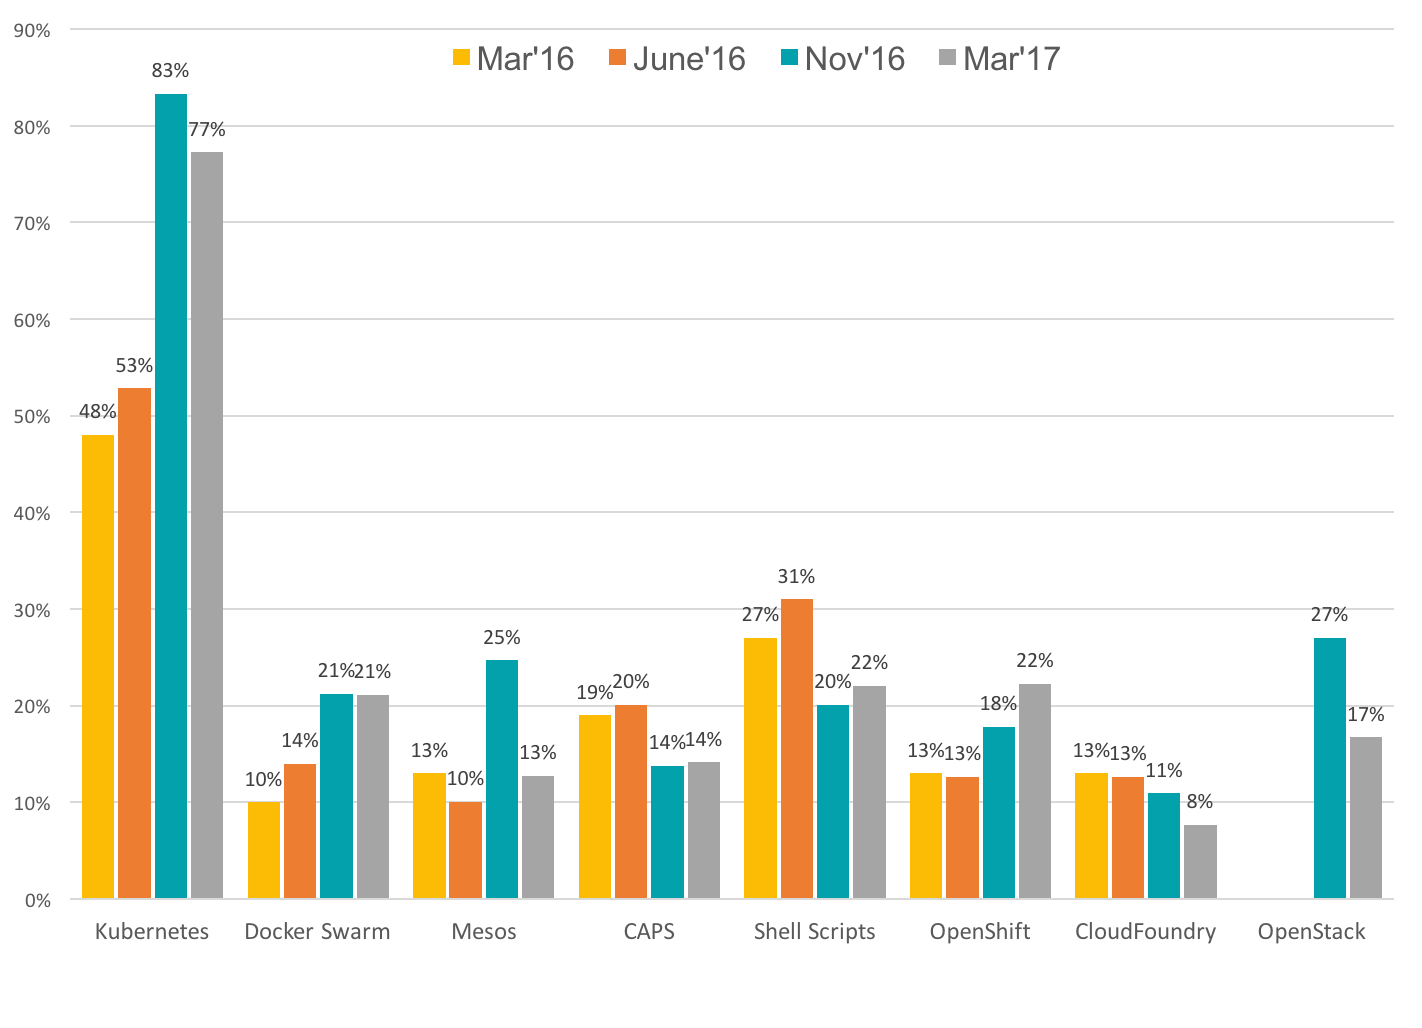
\includegraphics[width=7.5cm]{figures/cncf-container-orchestrators.png}
	%\caption{Preferred container management platforms, CNCF Survey, 2017}
	\label{fig:cncf-container-orchestrators}
	\\
	\tiny{Source: CNCF Survey, 2017}
\end{figure}
\end{frame}
%}}}
	
\begin{frame}{1.1 Topic and study scope - topic choice}%{{{
k8s is popular and used by practicioners
\begin{figure}
	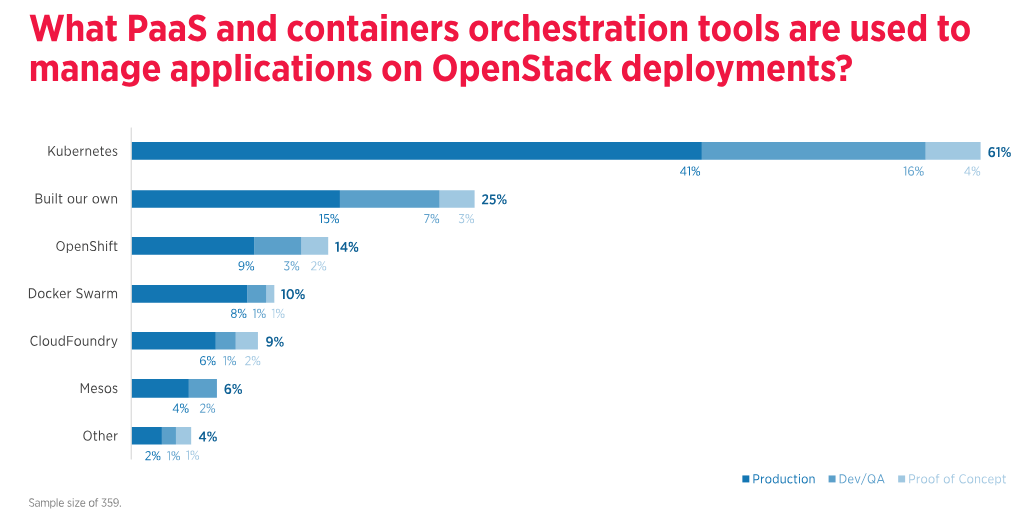
\includegraphics[width=10cm]{figures/k8s-openstack-survey.png}
	%\caption{Preferred containers orchestration tools on OpenStack, OpenStack Survey, 2018}
	\label{fig:k8s-openstack-survey}
	%\caption{Source: OpenStack Survey, 2018}
	\\
	\tiny{Source: OpenStack Survey, 2018}
\end{figure}
\end{frame}
%}}}
	
\begin{frame}{1.1 Topic and study scope - topic choice}%{{{
k8s is used in production environment
\begin{figure}
	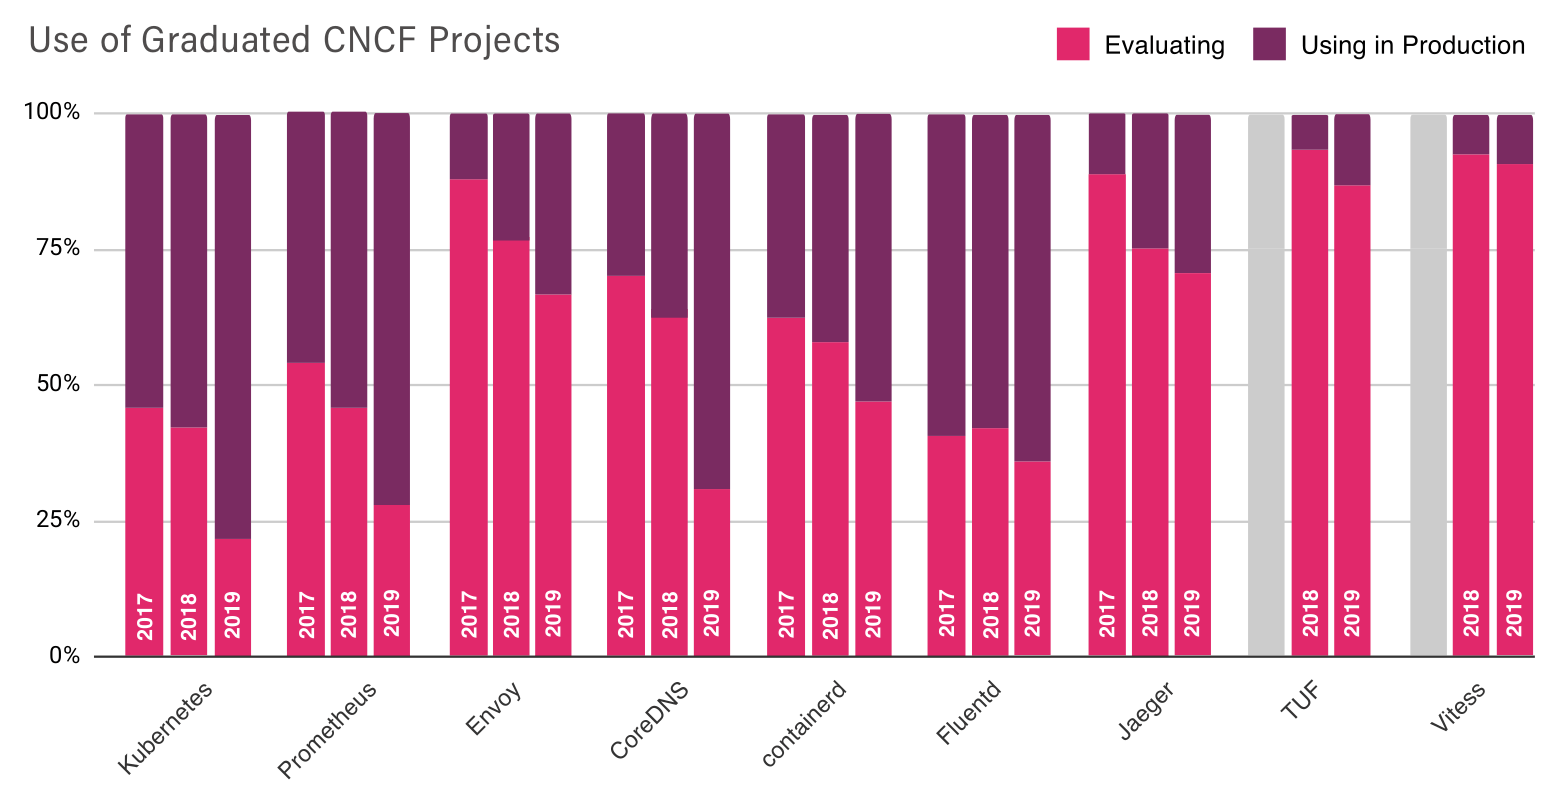
\includegraphics[width=10cm]{figures/cncf-k8s-used-in-production.png}
	\label{fig:cncf-k8s-used-in-production}
	\\
	\tiny{Source: CNCF Survey, 2019}
\end{figure}
\end{frame}
%}}}
	
\begin{frame}{1.1 Topic and study scope - topic choice}%{{{
k8s is used by NASA in production environment
\begin{center}
	\begin{figure}
		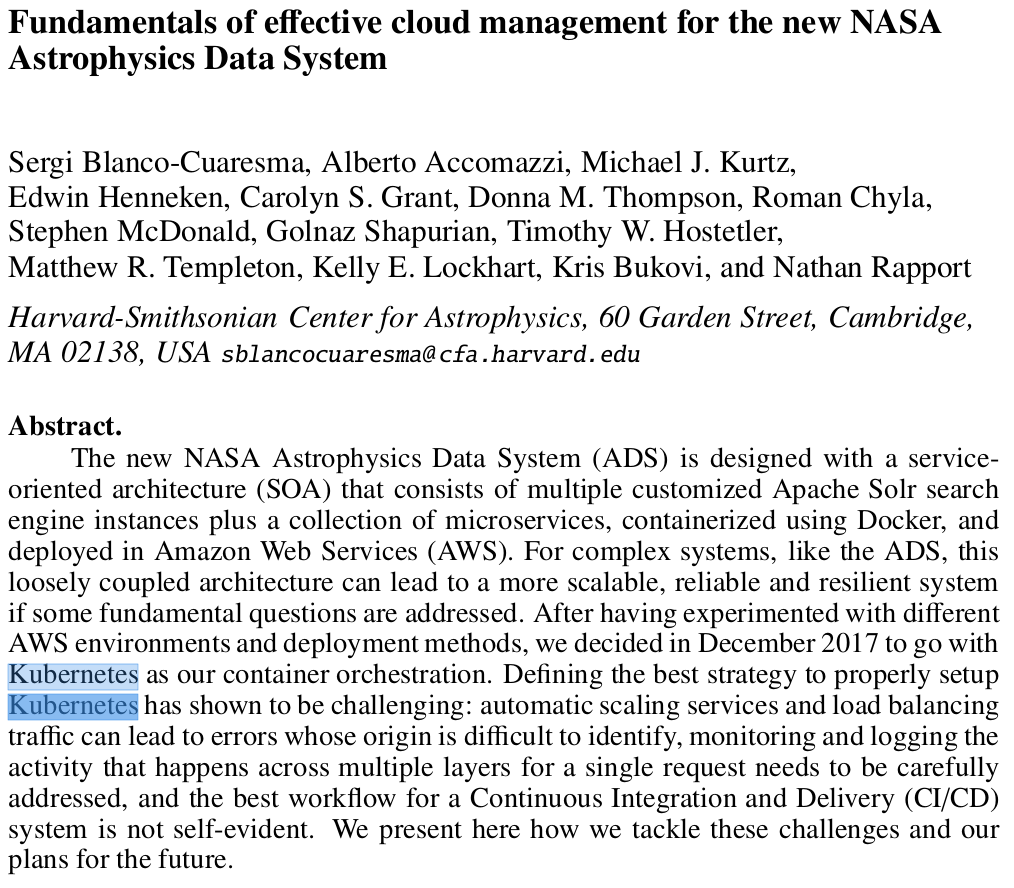
\includegraphics[width=6cm]{figures/k8s-used-by-nasa.png}
		\label{fig:k8s-used-by-nasa}
		\\
		\tiny{Blanco-Cuaresma, Sergi, et. al. \textit{Fundamentals of effective cloud management for the new NASA Astrophysics Data System}, 2019.}
	\end{figure}	
\end{center}
\end{frame}
%}}}

\begin{frame}{1.1 Topic and study scope - k8s deployment methods}%{{{
\begin{center}
	\begin{figure}
	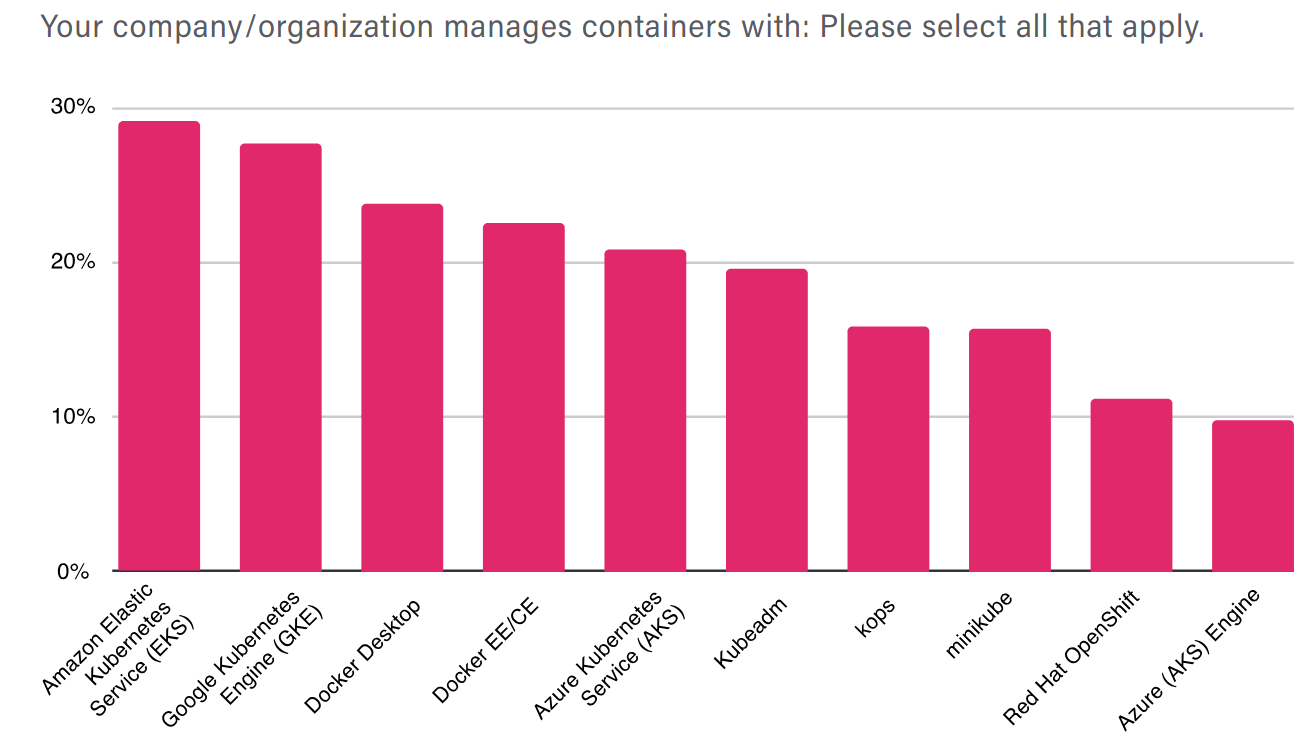
\includegraphics[width=8cm]{figures/cncf-k8s-deployment-methods.png}
	\label{fig:cncf-k8s-deployment-methods}
	\\
	\tiny{Source: CNCF Survey, 2019}
	\end{figure}	
\end{center}
\end{frame}
%}}}

\begin{frame}{1.1 Topic and study scope - topic choice}%{{{
The choice of \textbf{comparing two deployment methods on AWS}:
	\begin{itemize}
		\item Kubernetes cluster deployment methods are described by blog posts and tutorials - not formal literature, but \textbf{practitioners use them}
		\item Comparison of two deployment methods on AWS is \textbf{not found in literature} (however usage of Kubernetes cluster in production environment was handled)
		\item \textbf{AWS is a broadly adopted cloud} with long history
	\end{itemize}
\end{frame}
%}}}
	
\begin{frame}{1.1 Topic and study scope - topic choice}%{{{
The choice of \textbf{focusing on production environment}:
	\begin{itemize}
		\item To \textbf{facilitate others plan such deployment better} by letting them be aware upfront of its limitations and known issues
		\item To \textbf{apply a practical approach}
		\item Production environment is the one \textbf{creates value for businesses and customers}, it generates profit
		\item Because it is \textbf{challenging and interesting} to satisfy the requirements of a production environment
	\end{itemize}
\end{frame}
%}}}


\subsection{1.2 Aims and 1.3 Research Methodology}
\begin{frame}{1.2 Aims and 1.3 Research Methodology}%{{{
	\begin{itemize}
		\item Theoretical approach
		\begin{itemize}
			\item Search of existing literature (academic and other)
			\item Gather requirements of deployment in production environment
			\item Describe two deployment methods of Kubernetes cluster on AWS
		\end{itemize}
		\item Practical approach
		\begin{itemize}
			\item Perform the two deployments while conforming to the DevOps best practices and Agile methodology
			\item Compare these methods in the context of production environment
			\item List encountered problems and try to provide solutions
		\end{itemize}
	\end{itemize}
\end{frame}
%}}}


\subsection{1.4 Related work}
\begin{frame}{1.4 Related work - Formal literature}%{{{
\begin{itemize}
	\item Concern many clouds, practical approach, some production environment elements:
	\begin{itemize}
		\item \textbf{book}: Saito, Hideto. \textit{DevOps with Kubernetes: Accelerating software delivery with container orchestrators}. Packt Publishing, 2017. ISBN-13: 978-1788396646.
		\item \textbf{book}: Morris, Kief. \textit{Infrastructure as Code}. Edition 1. O'Reilly Media, 2016. ISBN-13: 978-1491924358.
		\item \textbf{book}: Sayfan, Gigi, et. al. \textit{Mastering Kubernetes}. Edition: 2.  Packt Publishing, 2018. ISBN-13: 978-1788999786.
	\end{itemize}
	\item \textbf{book}: Burns, Brendan, et. al. \textit{Kubernetes: Up and Running: Dive into the Future of Infrastructure}. Edition: 2. O'Reilly Media, 2019. ISBN-13: 978-1492046530. - many clouds, practical approach, no production environment elements
\end{itemize}
\end{frame}
%}}}
\begin{frame}{1.4 Related work - Formal literature cont.}%{{{
	\begin{itemize}
		\item \textbf{book}: Arundel, John, et. al. \textit{Cloud Native DevOps with Kubernetes: Building, Deploying, and Scaling Modern Applications in the Cloud}. Edition: 1. O'Reilly Media, 2019. ISBN-13: 978-1492040767. - many clouds, theoretical approach
		\item \textbf{book}: Source: Uphill, Thomas, et. al. \textit{DevOps: Puppet, Docker and Kubernetes}. Packt Publishing, 2017. ISBN 978-1788297615. - AWS, practical approach
		\item \textbf{papers} acknowledge using Kubernetes, but do not explain details of its deployment
	\end{itemize}
	\end{frame}
	%}}}

\begin{frame}{1.4 Related work - Informal literature}%{{{
\begin{itemize}
	\item \textbf{Many clouds compared, only theoretical approach}:
	\begin{itemize}
		\item https://platform9.com/blog/kubernetes-cloud-services-comparing-gke-eks-and-aks/
		\item https://logz.io/blog/kubernetes-as-a-service-gke-aks-eks/
		\item https://www.presslabs.com/blog/kubernetes-cloud-providers-2019/
	\end{itemize}
	\item \textbf{Practical approach, one method described}:
	\begin{itemize}
		\item https://eksctl.io/
		\item https://gruntwork.io/guides/kubernetes/how-to-deploy-production-grade-kubernetes-cluster-aws
		\item https://github.com/kelseyhightower/kubernetes-the-hard-way
		\item https://logz.io/blog/amazon-eks-cluster/
	\end{itemize}
\end{itemize}
\end{frame}
%}}}

\subsection{1.5 Structure of this thesis}
\begin{frame}{1.5 Structure of this thesis}%{{{
\begin{itemize}
	\item The 1st chapter serves as introduction and presents study topic, scope, aims, research methodology and related work  
	\item The chapters: 2. and 3. are theoretical 
	\item Chapter 2. focuses on definitions 
	\item Chapter 3. presents available k8s cluster deployment methods
	\item The chapters: 4., 5. and 6. are practical 
	\item Chapter 4. focuses on preparations before producing any code 
	\item Chapter 5. summarizes the deployment methods performed for this study by the author
	\item Chapter 6. compares the deployment methods 
	\item Chapter 7. provides a summary and future potential
\end{itemize}
\end{frame}
%}}}

\section{2. Definitions, 3. Available k8s cluster deployment methods}
\subsection{2.2 Production deployment requirements}
\begin{frame}{2.2 Production deployment requirements}%{{{
\begin{itemize}
	\item \textbf{Automation}
	\item \textbf{Security}
	\item \textbf{High Availability, failover, fault-tolerancy}
	\item \textbf{Backup and restore, Disaster Recovery}
	\item \textbf{Centralized Monitoring}
	\item \textbf{Centralized Logging}
	\item \textbf{Centralized Audit}
	\item \textbf{The k8s cluster must be healthy}
\end{itemize}
\\
\tiny{Source: Humble, Jez, et. al. \textit{Continuous Delivery}. Addison-Wesley, 2010. ISBN-13: 978-0321601919.}
\end{frame}
%}}}

\begin{frame}{2.2 Production deployment requirements - Automation}%{{{
\begin{itemize}
	\item Ensure \textbf{repetitive builds}, tests, deployments (Continuous Integration, Continuous Development)
	\item Apply \textbf{Infrastructure as Code}
	\item \textbf{Automated tests} that verify the \textbf{health of the k8s cluster}
\end{itemize}
\begin{figure}
	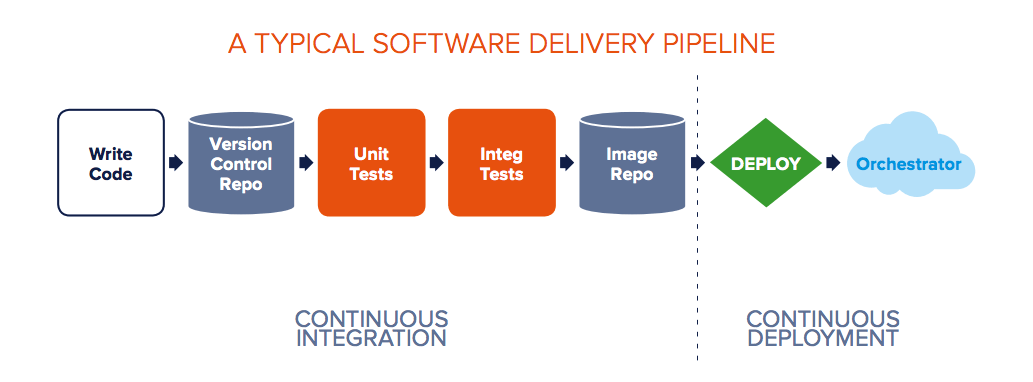
\includegraphics[width=8cm]{figures/cicd-pipeline.png}
	\label{fig:cicd-pipeline} \\
	\tiny{Source: \url{https://dzone.com/articles/5-steps-to-achieve-continuous-delivery}}
\end{figure}
\end{frame}

\begin{frame}{2.2 Production deployment requirements - Security}%{{{
\begin{itemize}
	\item Encryption in transit: HTTPS
	\item Use a static linter e.g. to check for hardcoded passwords or ssh keys
	\item RBAC, IAM - identity and access management on k8s AWS
\end{itemize}
\end{frame}
%}}}

\begin{frame}{2.2 Production deployment requirements - Monitoring}%{{{
\begin{itemize}
	\item Measuring the usage of CPU, Memory, IOPs, network usage, etc.
	\item Gather from many sources: including any APIs or services
	the application depends on
\end{itemize}
\begin{figure}
	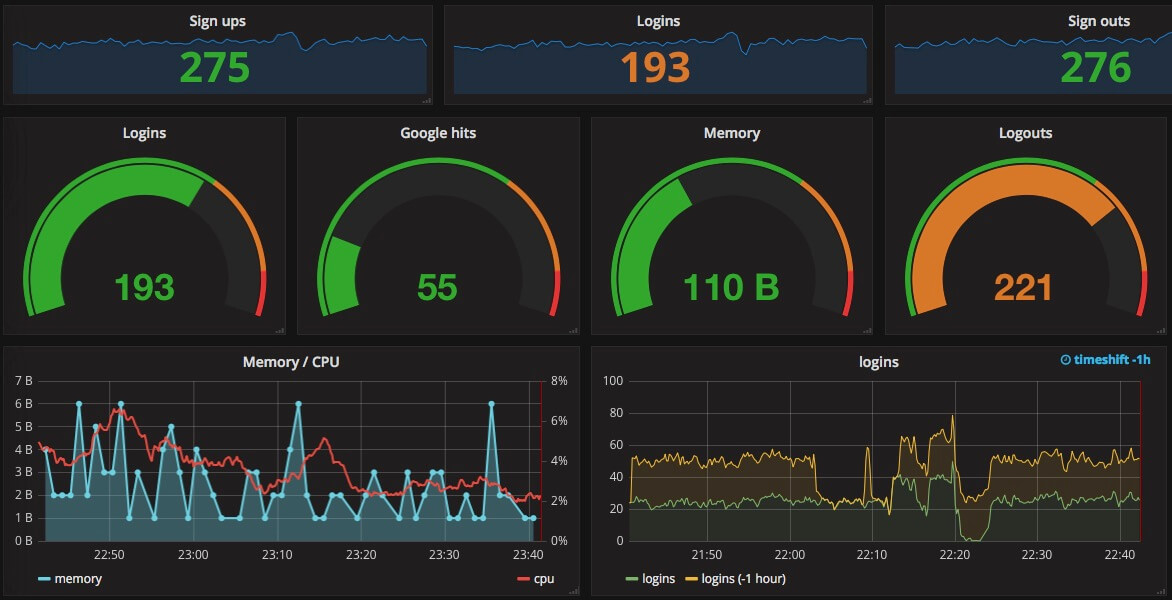
\includegraphics[width=7cm]{figures/grafana.jpeg}
	\label{fig:grafana} \\
	\tiny{Source: \url{http://codeblog.dotsandbrackets.com/wp-content/uploads/2017/01/grafana-dashboard.jpg}}
\end{figure}
\\
\end{frame}
%}}}

\subsection{2.5 Kubernetes architecture}
\begin{frame}{2.5 Kubernetes architecture}%{{{
\begin{figure}
	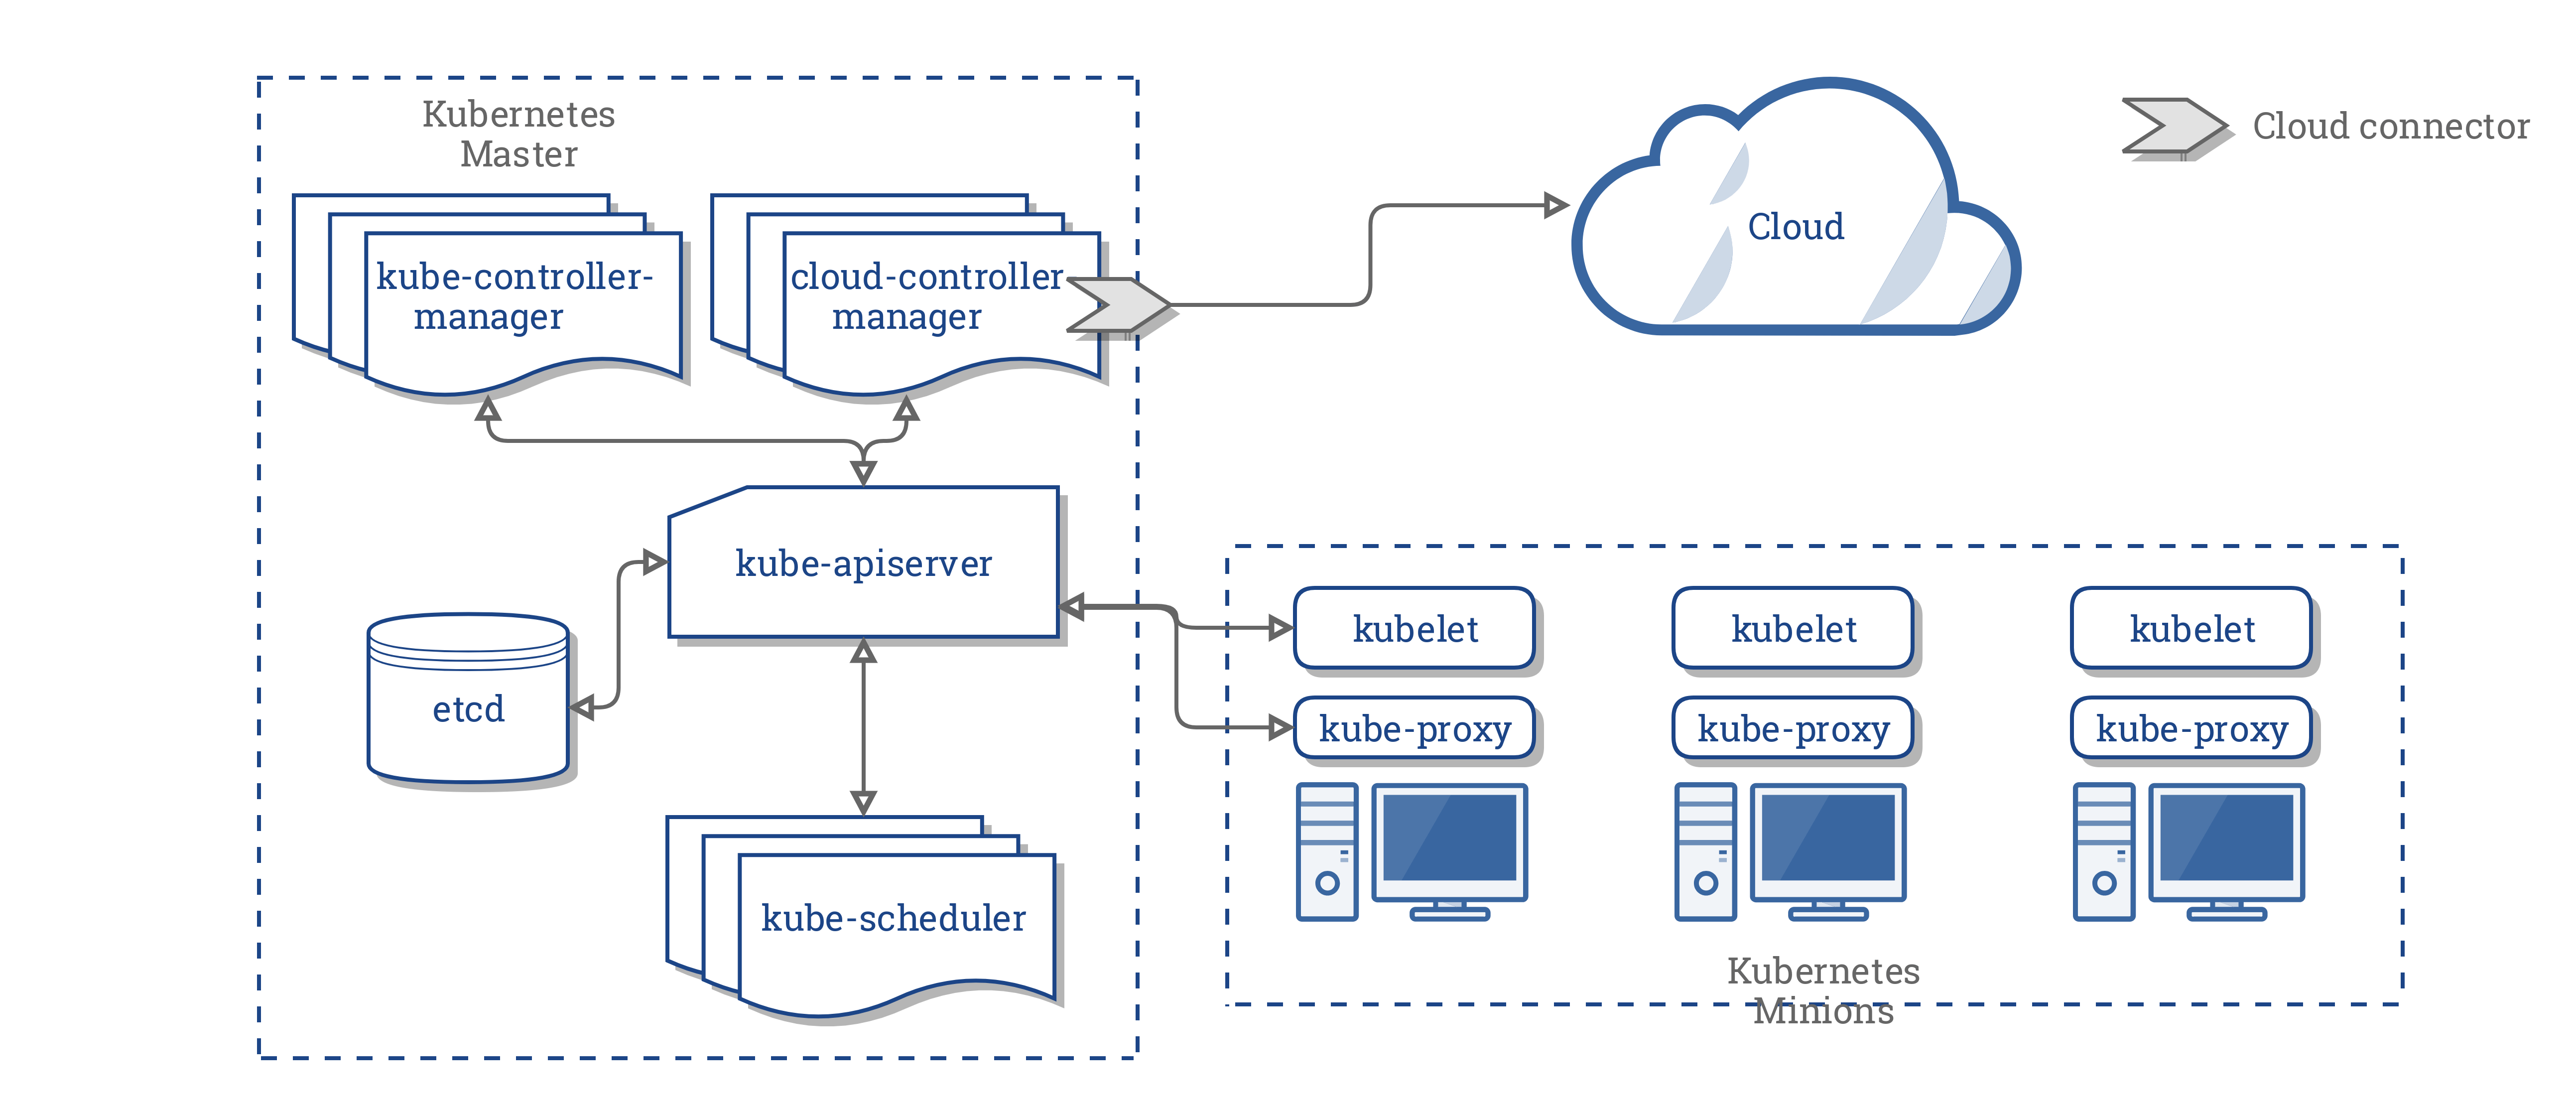
\includegraphics[width=10cm]{figures/k8s-arch.png}
	\label{fig:k8s-arch}
	\tiny{Source: https://kubernetes.io/docs/concepts/architecture/cloud-controller/}
\end{figure}
\end{frame}
%}}}

\subsection{3. k8s cluster deployment methods}
\begin{frame}{3. k8s cluster deployment methods - Managed k8s}%{{{
\begin{center}
	\begin{tabular}{ c c c}
		\begin{figure}
			
\includegraphics[width=3cm]{figures/managed-aws-eks.png}
			\label{fig:managed-aws-eks}
		\end{figure} &
		\begin{figure}
			
\includegraphics[width=3cm]{figures/managed-azure-kubernetes-service-aks.png}
			\label{fig:managed-azure-kubernetes-service-aks}
		\end{figure} &
		\begin{figure}
			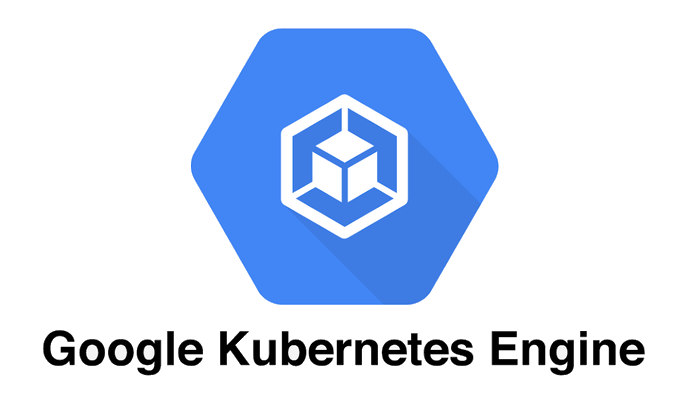
\includegraphics[width=4cm]{figures/managed-gcp-gke.png}
			\label{fig:managed-gcp-gke}
		\end{figure}
	\end{tabular}
\end{center}
\end{frame}
%}}}


\begin{frame}{3. k8s cluster deployment methods - custom solutions}%{{{
\begin{figure}
	
\includegraphics[width=11cm]{figures/custom-kops.png}
	\label{fig:custom-kops}
\end{figure}
\begin{figure}
	
\includegraphics[width=11cm]{figures/custom-kubeadm.png}
	\label{fig:custom-kubeadm}
\end{figure}
\begin{figure}
	
\includegraphics[width=11cm]{figures/custom-kubespray.png}
	\label{fig:custom-kubespray}
\end{figure}
\end{frame}
%}}}


\begin{frame}{3. k8s cluster deployment methods - custom solutions}%{{{
\begin{itemize}
	\item Configuration Management frameworks: SaltStack, Ansible, Chef, Puppet
	\item Infrastructure provisioning frameworks: Terraform, CloudFormation
\end{itemize}
\end{frame}
%}}}

\section{4. Preparations for production deployment of Kubernetes cluster}
\subsection{4.1 Chosen requirements of production deployment}
\begin{frame}{4.1 Chosen requirements of production deployment}%{{{
	\textit{this is just a draft!}
	\begin{itemize}
		\item Automation, Continuous Integration, Continuous Development, Infrastructure as Code
		\item Security
		\item High Availability, failover, fault-tolerancy
		\item Backup and restore, Disaster Recovery
		\item Centralized Monitoring
		\item Centralized Logging
		\item Centralized Audit
		\item The k8s cluster must be healthy
	\end{itemize}
\end{frame}

\subsection{4.2 Satisfying the automation requirement}
\begin{frame}{4.2 Satisfying the Automation requirement}%{{{
\begin{itemize}
	\item A CICD pipeline
	\item Design 2 environments: testing and production 
\end{itemize}
\end{frame}
%}}}
\begin{frame}{4.3 Satisfying the Security requirement}%{{{
	\begin{itemize}
		\item Encryption in transit: HTTPS
		\item Use a static linter e.g. to check for hardcoded passwords or ssh keys
		\item RBAC, IAM - identity and access management on k8s AWS
	\end{itemize}
\end{frame}
%}}}
\begin{frame}{4.4 Satisfying the High Availability (HA) requirement}%{{{
\begin{itemize}
	\item 3 Kubernetes master nodes? etcd as a cluster
	\item At least 2 worker nodes
	\item AWS ASG (auto scaling groups)
	\item Provide health checks to verify that cluster is up and running (healthy)
	\item Or: blue green deployments
	\item Test HA by introducing failures, measure the time needed to recover (compare with a paper)
\end{itemize}
\end{frame}
%}}}

\begin{frame}{4.5 Satisfying the Backup and Restore  requirement}%{{{
\begin{itemize}
	\item Automated script for etcd backup 
	\item Send backup outside
	\item Test the restore operation
\end{itemize}
\end{frame}
%}}}

\begin{frame}{4.6 Satisfying the Centralized Monitoring  requirement}%{{{
\begin{itemize}
	\item Use a server like Nagios, Grafana, InfluxDB, Prometheus, etc.
	\item Use some AWS service e.g. CloudWatch
\end{itemize}
\end{frame}
%}}}

\begin{frame}{4.7 Satisfying the Centralized Logging  requirement}%{{{
\begin{itemize}
	\item Use a server like Graylog, Fluentd, LogStash
	\item Use some AWS service e.g. CloudWatch
\end{itemize}
\end{frame}
%}}}

\begin{frame}{4.8 Satisfying the Centralized Audit requirement}%{{{
\begin{itemize}
	\item Use some AWS service e.g. CloudTrail, AWS Config
	\item Allow access to production only through CICD pipeline
	\item Some k8s built-in solution? cloud agnostic method
\end{itemize}
\end{frame}
%}}}

\begin{frame}{4.9 Verifying that k8s cluster is healthy}%{{{
\begin{itemize}
	\item Check health status of all k8s services
	\item Use a status dashboard
	\item Check it every 1 minute
	\item Deploy a small app on k8s to test that k8s is usable
	\item Run these tests also in a CICD pipeline
\end{itemize}
\end{frame}
%}}}

\section{5. Production deployment, 6. Comparison}
\subsection{5.1 Production deployment - using method: AWS EKS}
\begin{frame}{5.1 Production deployment - using method: AWS EKS}%{{{
\begin{itemize}
	\item Link to code
	\item Main steps summarized
	\item Overall how it went
	\item Some problems + solutions 
\end{itemize}
\end{frame}
%}}}

\subsection{5.2 Production deployment - using method: AWS with Kops}
\begin{frame}{5.2 Production deployment - using method: AWS with Kops}%{{{
\begin{itemize}
	\item Link to code
	\item Main steps summarized
	\item Overall how it went
	\item Some problems + solutions 
\end{itemize}
\end{frame}
%}}}

\subsection{6. Comparison}
\begin{frame}{6.1 Criterium 1: Cost}%{{{

\end{frame}
%}}}

\begin{frame}{6.2 Criterium 2: The amount of problems}%{{{

\end{frame}
%}}}

\begin{frame}{6.3 Criterium 3: The amount of not automated resources}%{{{

\end{frame}
%}}}

\begin{frame}{6.4 - Criterium 4: Production deployment requirements met?}%{{{

\end{frame}
%}}}

\subsection{6.5 Comparison summary}
\begin{frame}{6.5 Comparison summary}%{{{
	\begin{tabular}{| l | c | c |}
		\hline
		& AWS EKS & AWS Kops \\
		\hline
		Cost &  &  \\
		\hline
		Problems count &  &  \\
		\hline
		Not automated resources count &  &  \\
		\hline
		Production requirements met &  &  \\
		\hline
		\end{tabular}
\end{frame}
%}}}

\section{7. Summary, 8. Literature}
\subsection{7.1 Lessons learned and achieved results}
\begin{frame}{7.1 Lessons learned and achieved results}%{{{
\begin{itemize}
	\item Choose which method was better, applying specified criteria 
	\item Maybe some more preparations were needed - more planning, design
\end{itemize}
\end{frame}
%}}}
\subsection{7.2 Future work potential}
\begin{frame}{7.2 Future work potential}%{{{
\begin{itemize}
	\item Compare more methods of deployment
	\item Use more comparison criteria 
	\item Use more production requirements, e.g. automated upgrades
	\item Apply more load and run load and performance tests
	\item Instead of satisfying production requirements, test enterprise and big data deployments requirements - create a survey to get lessons learned based on long running clusters and their administration
\end{itemize}
\end{frame}
%}}}
\subsection{8. Literature}
\begin{frame}{8. Literature}%{{{
	\tiny{
\begin{itemize}
	\item Uphill, Thomas, et. al. \textit{DevOps: Puppet, Docker and Kubernetes}. Packt Publishing, 2017. ISBN 978-1788297615
	\item Alonso, Ruben. \textit{Software containerization with Docker}. Bachelor's thesis. Turku University of Applied Sciences, 2017.
	\item Saito, Hideto. \textit{DevOps with Kubernetes: Accelerating software delivery with container orchestrators}. Packt Publishing, 2017. ISBN-13: 978-1788396646.
	\item Morris, Kief. \textit{Infrastructure as Code}. Edition 1. O'Reilly Media, 2016. ISBN-13: 978-1491924358.
	\item Nemer, Joe. \textit{Advantages and Disadvantages of Microservices Architecture}. Cloud Academy, 2019. [Accessed: 06.04.2020] Available at: https://cloudacademy.com/blog/microservices-architecture-challenge-advantage-drawback/
	\item Balalaie, Armin, et. al. \textit{Microservices Architecture Enables DevOps: An Experience Report on Migration to a Cloud-Native Architecture}. IEEE Software, 2016, vol. 33.
	\item https://continuousdelivery.com/ [Accessed: 06.04.2020]
	\item Humble, Jez, et. al. \textit{Continuous Delivery}. Addison-Wesley, 2010. ISBN-13: 978-0321601919.
	\item Burns, Brendan, et. al. \textit{Kubernetes: Up and Running: Dive into the Future of Infrastructure}. Edition: 2. O'Reilly Media, 2019. ISBN-13: 978-1492046530.
	\item Blanco-Cuaresma, Sergi, et. al. \textit{Fundamentals of effective cloud management for the new NASA Astrophysics Data System}, 2019.
	\item Arundel, John, et. al. \textit{Cloud Native DevOps with Kubernetes: Building, Deploying, and Scaling Modern Applications in the Cloud}. Edition: 1. O'Reilly Media, 2019. ISBN-13: 978-1492040767.
	\item Sayfan, Gigi, et. al. \textit{Mastering Kubernetes}. Edition: 2.  Packt Publishing, 2018. ISBN-13: 978-1788999786.
\end{itemize}
	}
\end{frame}
%}}}


\begin{frame}{8. Literature}%{{{
	\tiny{
\begin{itemize}
\item \url{https://docs.docker.com}
\item \url{https://platform9.com/blog/kubernetes-cloud-services-comparing-gke-eks-and-aks/}
\item \url{https://logz.io/blog/kubernetes-as-a-service-gke-aks-eks/}
\item \url{https://www.presslabs.com/blog/kubernetes-cloud-providers-2019/}
\item \url{https://eksctl.io/}
\item \url{https://gruntwork.io/guides/kubernetes/how-to-deploy-production-grade-kubernetes-cluster-aws}
\item \url{https://github.com/kelseyhightower/kubernetes-the-hard-way}
\item \url{https://logz.io/blog/amazon-eks-cluster/}
\item \url{https://microservices.io/}
\end{itemize}
	}
\end{frame}
%}}}

\end{document}

